\documentclass[a4paper,twoside,kulak]{kulakreport} %options: kul or kulak (default)

\usepackage[utf8]{inputenc}
\usepackage[dutch]{babel}
\usepackage{eurosym}
\usepackage[utf8]{inputenc}
\usepackage[dutch]{babel}
\usepackage{siunitx}
\usepackage{graphicx}
\usepackage{flafter}
\usepackage{pdfpages}
\usepackage{caption}
\usepackage{subcaption}
\usepackage{booktabs}
\usepackage{url}
\usepackage{hyperref}





\faculty{Wetenschap \& Technologie Kulak}
\group{Ingenieurswetenschappen}
\title{How to make \textit{an automated microplate dispenser}}
\subtitle{Een zoektocht naar balans tussen precisie, snelheid en betaalbaarheid}
\author{Team ELISA}
\institute{Matthias Derez, Maxime Dujardin, Korneel Verkens, Seppe Vilain}
\date{Academiejaar 2019 -- 2020}
\address{
   KU Leuven Kulak           \\
   Wetenschap \& Technologie \\
   Etienne Sabbelaan 53, 8500 Kortrijk                \\
   
   }

\begin{document} % hier begint de eigenlijke inhoud van het document
\sffamily
\titlepage

\tableofcontents

\chapter*{Inleiding}
Vandaag de dag komen veel mensen in contact met HIV, de ziekte van Lyme en voedselallergenen. Om deze aandoeningen op te sporen, kan de ELISA-test (\textit{Enzyme-Linked ImmunoSorbent Assay}) gebruikt worden. Het is een laboratoriumtest die gebruikt wordt voor het meten van macromoleculaire stoffen in bloedmonsters. Door, gebruik makend van een enzym als merker, een specifieke antigeen-antistofbinding aan te tonen in het bloed of andere lichaamsvloeistof van een mens of dier, kan de eventuele aanwezigheid van de aandoening vastgesteld worden. 
\newline
Beeld je in dat je een gedreven laborant bent die werkt met de ELISA-test en op zoek is naar de aandoening waaraan een patiënt lijdt. Je wil dan natuurlijk liefst zo veel mogelijk tijd en moeite steken in de analyse van de chemische stoffen en geen kostbare tijd verliezen aan het voortdurend handmatig titreren van de stoffen in de \textit{microplate} zoals dit nu gebeurt in het\textit{Laboratory for Thrombosis Research} aan Kulak. De \textit{automatic microplate dispenser} is hiervoor de oplossing. Deze machine is snel en niet moe te maken, waardoor fouten uitgesloten worden. Mede door deze voordelen zal de \textit{automatic microplate dispenser} op termijn niet meer weg te denken zijn uit moderne laboratoria en zal deze mee zijn stempel drukken op de vooruitgang van de geneeskunde. Het grote probleem aan de \textit{automated microplate dispensers} die momenteel op de markt zijn, is dat prijzen voor een tweedehandstoestel beginnen bij \euro 1500 à \euro 8500. Omdat dit veel geld is voor een machine die eigenlijk een relatief simpele handeling, besloten wij, studenten Ingenieurswetenschappen, zelf een machine te maken die hetzelfde doet als de apparaten die momenteel op de markt zijn, maar dan voor een wél acceptabele prijs.


\chapter{Klantenvereisten}
De klant wil een geautomatiseerde \textit{dispenser}. De \textit{dispenser} moet in staat zijn om volledig autonoom een \textit{microwell}-plaat te vullen met de te onderzoeken substantie. Dit proces moet foutloos gebeuren: in elke \textit{microwell} moet exact evenveel substantie zitten en er mag niet naast de \textit{microwells} gemorst worden. Bovendien moet dit alles kunnen in een tijd die aanzienlijk korter is dan wanneer men deze \textit{microwell}-plaat handmatig zou vullen. Vooral dit laatse aspect is belangrijk, aangezien het handmatig vullen van de platen een zeer arbeidsintensief en tijdrovend onderdeel is van de ELISA-test. Het apparaat moet eenvoudig te bedienen zijn en de pipetpunten die de substantie in de \textit{wells} spuiten, moeten vervangbaar zijn.  Indien mogelijk kunnen ook al andere stappen, buiten het vullen van de \textit{microwells} zelf, geautomatiseerd worden. Het automatisch aan- en afvoeren van \textit{microwell}-platen kan het productieproces al veel versnellen. Er is een budget van \EUR{50} tot \EUR{75} voorzien.
\chapter{Ontwerpspecificaties}
De te onderzoeken substantie bevindt zich in een recipiënt van waaruit het kan worden opgezogen. De \textit{microwell}-plaat is 27.76 mm breed, 85.48 mm lang en 14.4 mm hoog. Er zitten 96 \textit{microwells} in, met een bovendiameter van 6.96 mm en een benedendiameter van 6.58 mm (zie Figuur \ref{fig: afmetingenMicrowellplaat}). Het werkvolume van elke \textit{well} is tussen 25 $\mu l$ en 340 $\mu l$. De middelpunten van de \textit{wells} bevinden zich op 9 mm van elkaar. De middelpunten van de pipetpunten moeten dus op 9 mm van elkaar zitten en moeten verwijderbaar zijn. De machine moet elke \textit{well} kunnen vullen met een hoeveelheid van 100 $\mu l$ of 200 $\mu l$ van de te onderzoeken substantie. Om de vloeistof niet te morsen naast de \textit{wells}, moeten de pipetpunten telkens exact boven het middelpunt van de \textit{well} de vloeistof lossen. Om het apparaat gebruiksvriendelijk te maken, moet een grafische interface voorzien worden. Zo kan de machine in enkele tellen opgestart worden en kunnen onderzoekers die de programmeertaal niet kennen de machine toch zonder probleem gebruiken.

\begin{figure}[h]
	\centering
	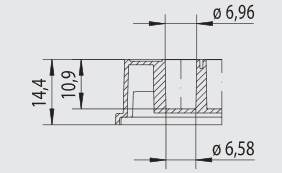
\includegraphics[width=0.5\textwidth]{AfmetingenMicrowell.png}
	\caption{Afmetingen \textit{microwell}}
	\label{fig: afmetingenMicrowellplaat}
	
\end{figure} 


\chapter{Ontwerp} 


In deze sectie wordt het uiteindelijke concept toegelicht en uitgelegd waarom dit concept weerhouden is.

\section{Werking}

	Het concept (zie Figuren \ref{fig: CAD-model globaal} en \ref{fig: CAD-model ingezoomd}) laat toe om zes \textit{microwell}-platen in één keer te vullen.  Er wordt gewerkt met een pomp die de vloeistof uit het recipiënt oppompt en via een buizennetwerk verdeelt over acht pipetpunten waarvan de middelpunten zich op een afstand van 9 mm van elkaar bevinden. De verdeling gebeurt door elke buis te splitsen in twee andere buizen m.b.v. een verdeelstuk. De pipetpunten kunnen van de machine gehaald worden en zo gemakkelijk vervangen worden. In het platform waar de \textit{microwell}-platen worden op geplaatst, zitten zes rechthoeken in de vorm van de \textit{microwell}-platen gefreesd zodat de platen vastzitten. Het platform is vastgemaakt aan een aandrijfriem en \textit{stepper}-motor en kan op die manier verplaatst worden. Telkens wanneer een rij van acht \textit{wells} gevuld is, stopt de pomp en verschuift de \textit{microwell}-plaat 9 mm naar links. Daarna vult de pomp opnieuw acht \textit{wells}. Dit proces wordt herhaald tot de twaalf rijen van acht \textit{wells} gevuld zijn. 
	
\section{Voordelen}
	We gebruiken slechts 8 pipetpunten en geen 12 of 96. Er werd beslist om geen 96 \textit{wells} tegelijk te vullen omdat één enkele pomp niet genoeg zuigkracht genereert om zo'n grote hoeveelheid vloeistof te kunnen opzuigen. De reden dat we geen 12 \textit{wells} tegelijk vullen is de volgende: wanneer we de vloeistof verdelen over 8 pipetpunten, kunnen we ervoor zorgen dat de vloeistof van het recipiënt tot aan elk van de 8 pipetpunten een gelijke afstand aflegt. Dit kan eenvoudig gerealiseerd worden door de buizen te verdelen m.b.v. T- of Y-verdeelstukken, wat bij 12 pipetpunten niet het geval is. Dit laatste zou ervoor kunnen zorgen dat er niet evenveel vloeistof in elke \textit{well} komt, wat problemen oplevert bij het uitvoeren van de ELISA-test. Dit concept heeft ook als voordeel t.o.v. andere concepten die opgesteld werden dat er maar één bewegend onderdeel is. Hierdoor kan het aantal motoren beperkt worden. Een ander voordeel van dit concept is dat het relatief goedkoop is. Bij andere concepten die gemaakt werden, werd voorgesteld om met cilinders en zuigers te werken i.p.v. met een pomp. Deze onderdelen kosten per stuk echter even veel als het voorziene budget voor dit project. Door met een pomp te werken kan dit vermeden worden en wordt de kostprijs aanzienlijk gedrukt. 
	
\begin{figure}[h]
	\centering
	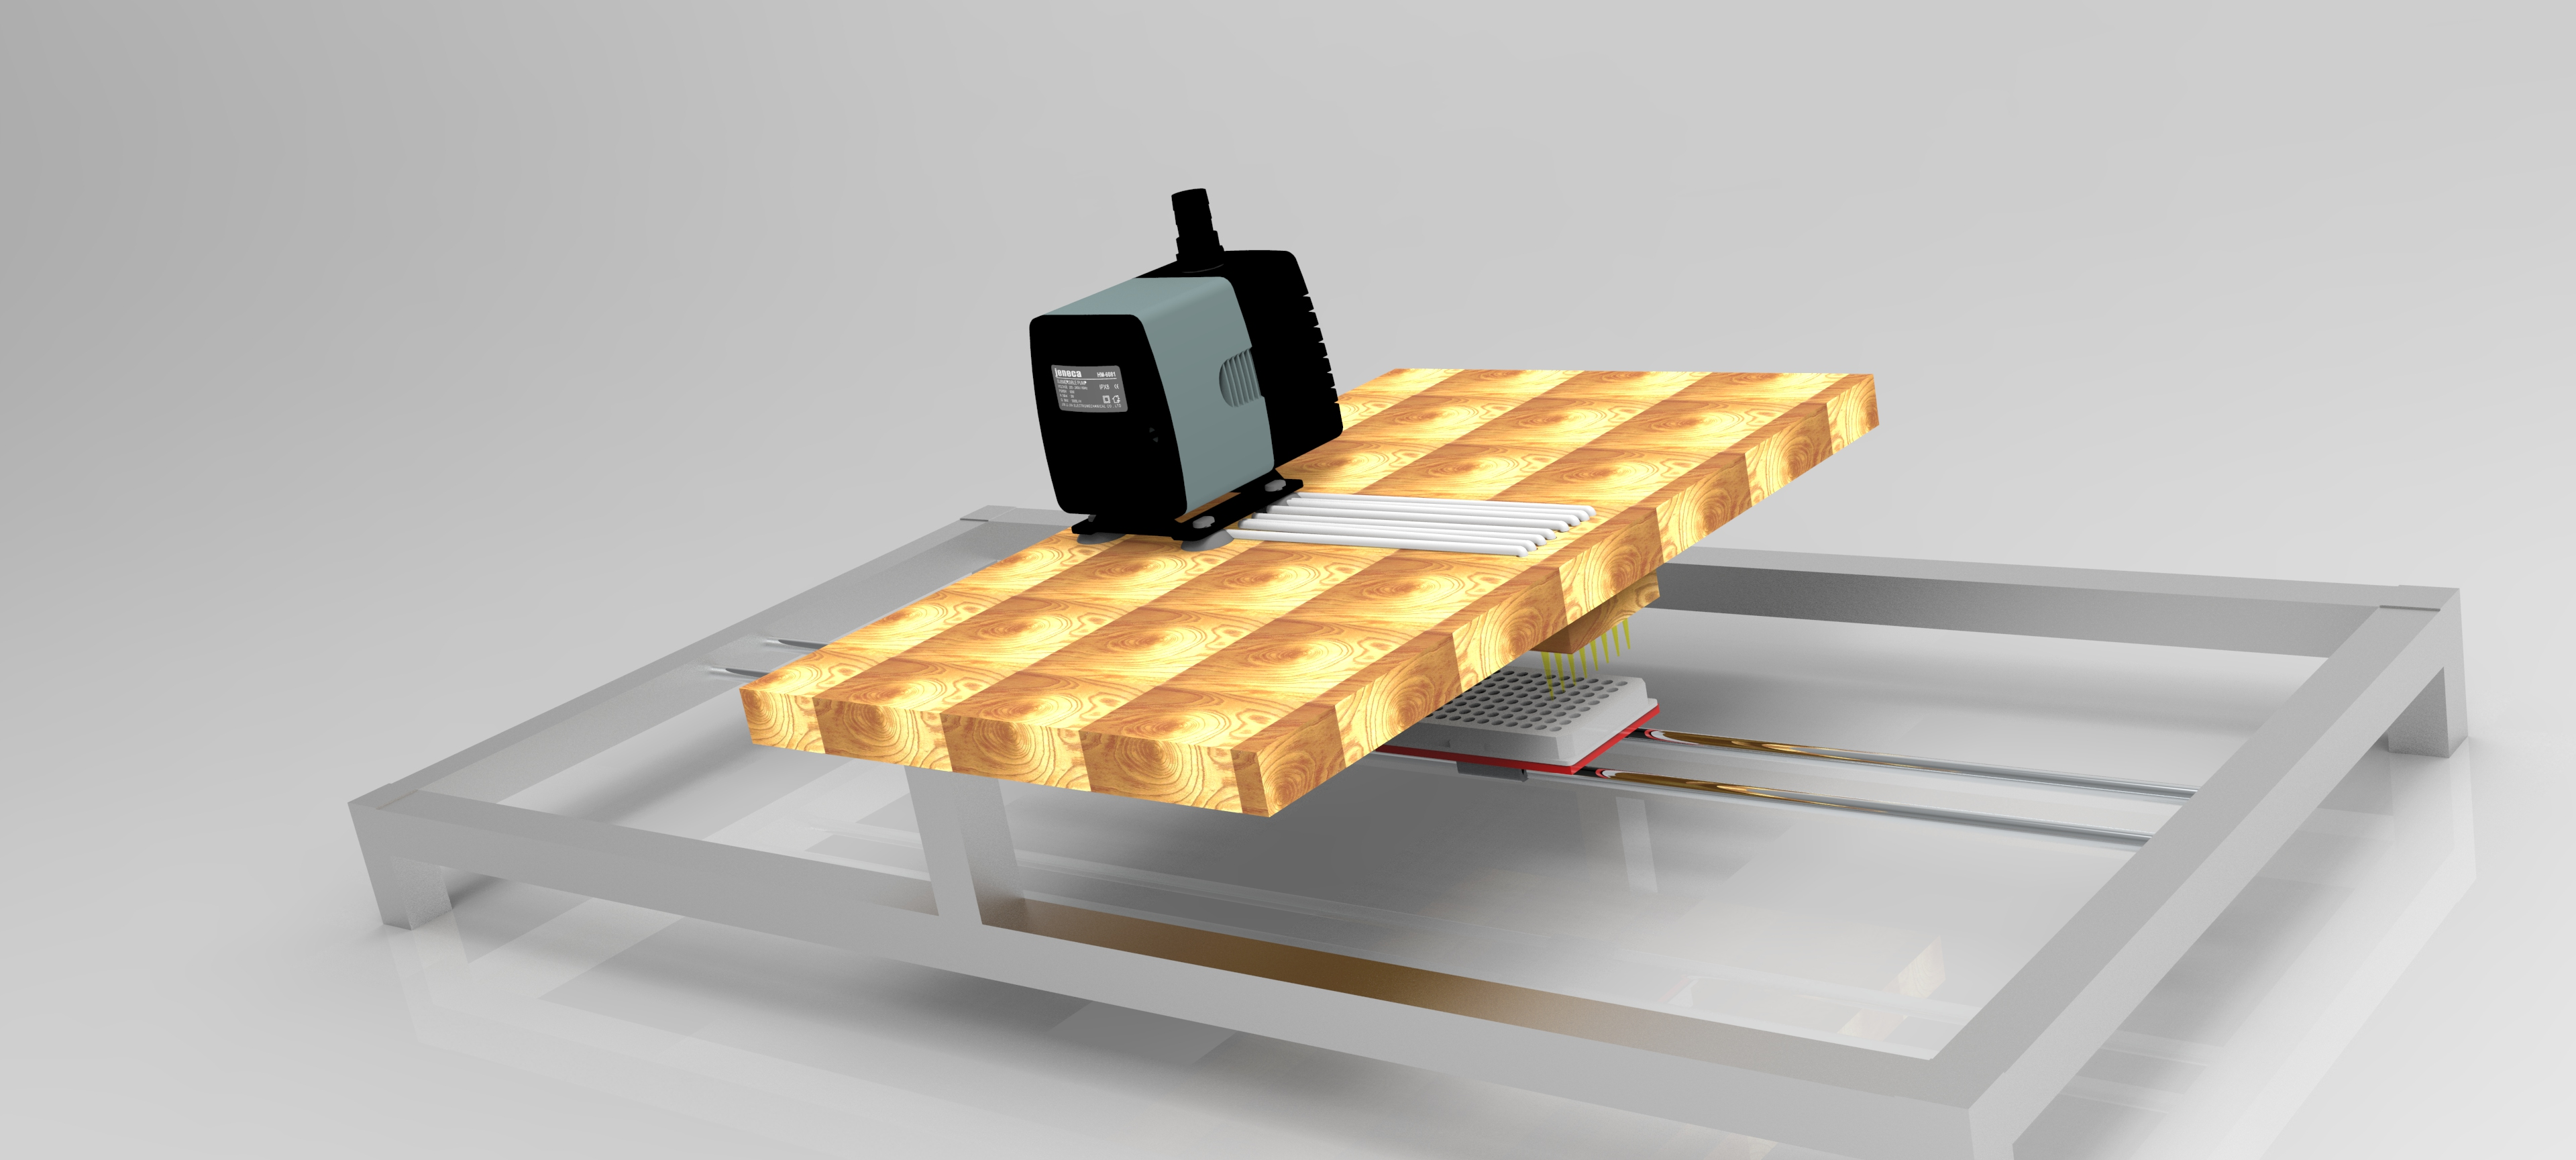
\includegraphics[width=0.8\textwidth]{micdis1.jpg}
	\caption{CAD-model concept 3}
	\label{fig: CAD-model globaal}
	
\end{figure} 

\begin{figure}[h]
	\centering
	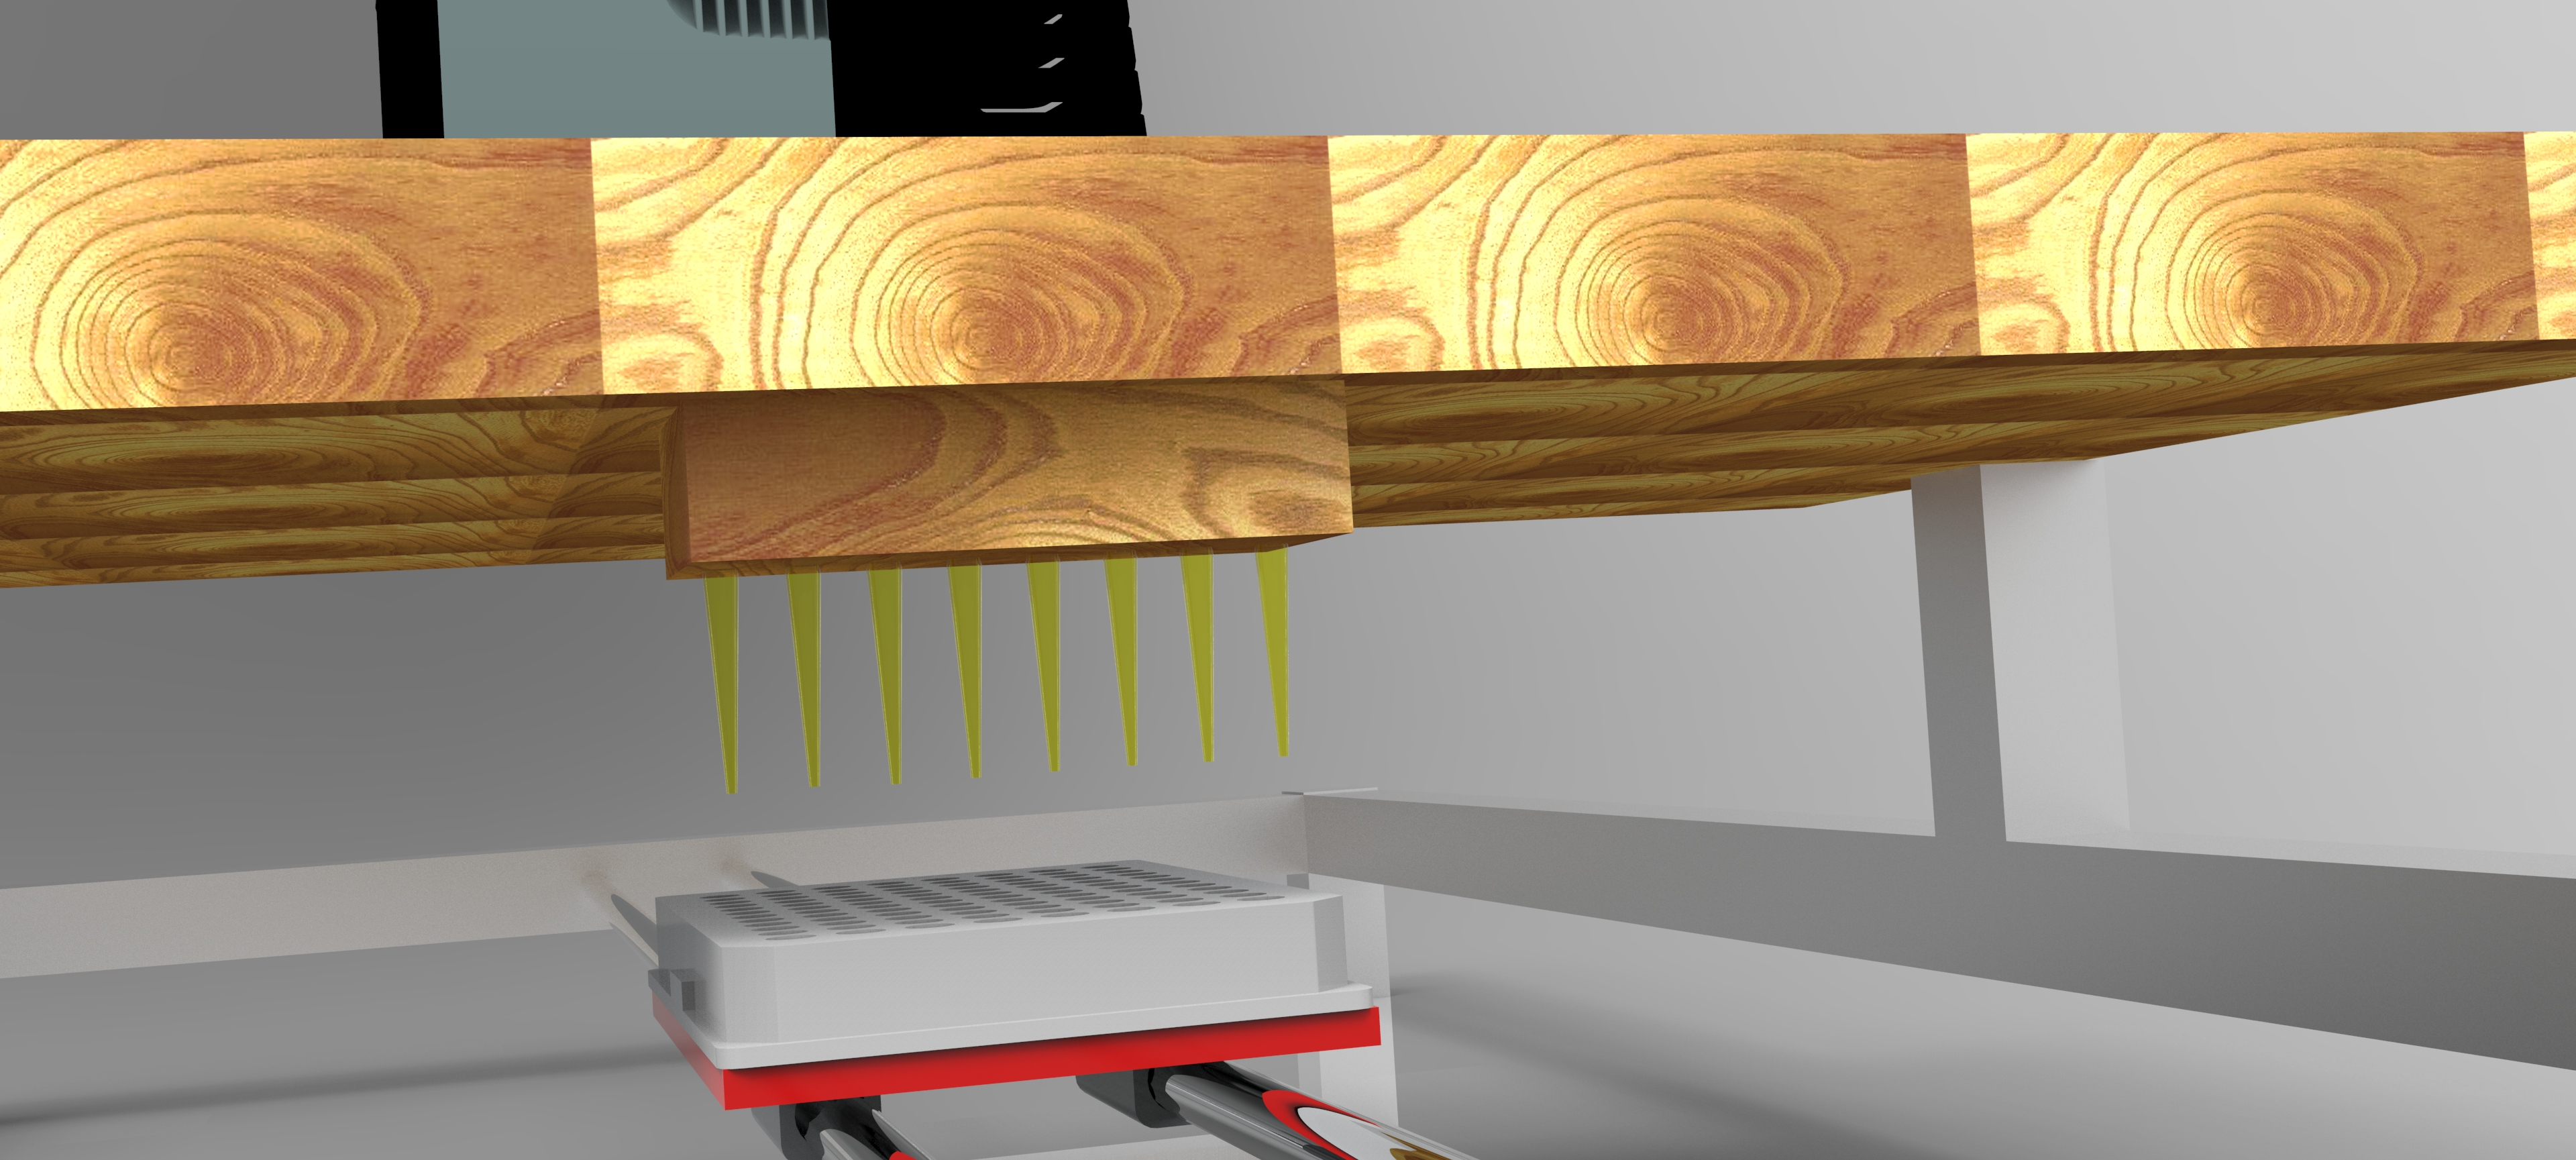
\includegraphics[width=0.8\textwidth]{micdis2.jpg}
	\caption{CAD-model concept 3}
	\label{fig: CAD-model ingezoomd}
	
\end{figure} 


\chapter{\textit{Unique selling point}}

De door ons gebouwde machine heeft heel wat potentieel. Hieronder vindt u enkele grote pluspunten die onze machine onderscheidt van toestellen die reeds op de markt zijn.

\paragraph{Prijs-kwaliteitverhouding}

Het grootste voordeel van ons toestel t.o.v. andere toestellen is ongetwijfeld de uitstekende prijs-kwaliteitverhouding. Ons toestel kost in totaal \euro BEDRAG (dit is weliswaar zonder werkuren te verrekenen), wat 5 tot 10 keer minder is dan de prijs van andere toestellen. De machine werkt precies en snel, precies wat er verwacht wordt van een dergelijk apparaat. Kortom: de prijs-kwaliteitverhouding is uitstekend.

\paragraph{Gebruiksgemak}

Doordat alles geautomatiseerd is, hoeft de gebruiker van het apparaat zeer weinig te doen om de \textit{microwell}-platen te vullen. Men hoeft enkel het aantal te vullen \textit{microwell}-platen en het volume per \textit{microwell} te specifiëren en de \textit{microwell}-platen op de transportband te plaatsen. Het ingeven van de aantallen en volumes kan heel snel en eenvoudig gebeuren via DRUKKNOPPEN OF INTERFACE.

\paragraph{Mobiliteit en stevigheid}

Tijdens het ontwerp en materiaalkeuze werd zo veel mogelijk rekeing gehouden met de massa van het toestel. De gehele machine is gebouwd op een chassis uit aluminium om een stevige basis te bekomen. Het platform op het chassis werd vervaardigd uit hout om zo veel mogelijk gewicht te besparen. Dit levert een licht, maar zeer stevig geheel op. 

\paragraph{Veiligheid}
VERMELDEN DAT ER DETECTOREN EN STOPKNOPPEN ZITTEN AAN DE TWEE UITEINDEN?

\paragraph{Hygiëne}

Een mogelijk nadeel van hout is dat het kan rotten wanneer er vloeistoffen op gemorst worden. Dit wordt echter verholpen door een beschermende coating aan te brengen die het hout beschermt tegen vloeistoffen. Dit zorgt er tevens voor dat de machine gereinigd kan worden zonder dat de onderdelen hieronder lijden.

\paragraph{Vervangstukken}

De machine werd gemaakt uit onderdelen die gemakkelijk te vinden zijn in zowel winkels als op internet. Dit zorgt ervoor dat de gebruiker in het geval van een defect onderdeel snel kan geholpen worden en snel weer aan de slag kan.

\chapter{Mogelijkheden tot uitbreiding}
platen automatisch erop zetten
\chapter*{Appendices}
\section*{Financieel verslag}

In Tabel \ref{tab:financieelVerslag} staan de gemaakte aankopen vermeld. 


\begin{table}[!hbt]
	\noindent\makebox[\textwidth]
	\sffamily
	
	\caption{Aankopen}
		\begin{tabular}{@{}lllll@{}}
		\toprule
		  Item & Product & Prijs/stuk (\euro) & Aantal & Totaal (\euro)   \\ \midrule
		1 & Staaf voor X- of Y-as glad 10 mm x 100 cm & 4.75 & 2 & 9.50 \\
		2 & SCS10UU lineaire kogellager  & 5.50 & 2 & 11.00 \\
		3 & GT2 timing belt 6 mm (per meter)  & 4.50 & 2 & 9.00 \\
		4 & GT2 Pulley hoge resolutie | 6 mm riem | 20 tanden | 5 mm as & 6.00 & 1 & 6.00 \\
		5 & Spanrol | gladde pulley hoge resolutie | 6 mm riem | 5 mm as & 5.50 & 1 & 5.50 \\
		6 & SHF10 as-bevestiging (2 stuks) & 9.50 & 2 & 19.00 \\
		7 & Aluminium profiel 2020 extrusion lengte 1 m (123-3D huismerk)  & 9.50 & 3 & 28.50 \\
		8 & Aluminium hoekverbinding 2020 inclusief bevestigingsmateriaal (123-3D huismerk) & 2.75 & 4 & 11.00 \\
		9 & Hulpstukje 4 mm Luchtslang PE T-stuk 4 x 4 x 4 mm & 0.20 & 15 & 3.00 \\
		\bottomrule
	\end{tabular}
	\label{tab:financieelVerslag}

	
\end{table}


\clearpage

\section*{Verantwoordelijkheden taakverdeling}

De volledige opdracht werd verdeeld in volgende delen (met bijhorende verantwoordelijken):
\begin{itemize}
	\item \textsc{Teamleider:} Seppe Vilain
	\item \textsc{Notulist}: Maxime Dujardin
	\item \textsc{Opstellen CAD-model}: Korneel Verkens
	\item \textsc{Mechanisme om platform met \textit{microwell}-platen te verplaatsen:} Matthias Derez, Seppe Vilain
	\item \textsc{Pompsysteem:} Maxime Dujardin, Korneel Verkens
	\item \textsc{Verslag \& presentatie:} Matthias Derez, Maxime Dujardin, Korneel Verkens, Seppe Vilain
	
\end{itemize}

\clearpage

\section*{Vakintegratie}
Om dit project tot een goed einde te kunnen brengen werden een aantal vakken uit semesters 1 t.e.m. 3 gebruikt:

\paragraph{Algemene Natuurkunde: Mechanica}

In het vak 'Mechanica' werden de basisbeginselen i.v.m. druk en stroming in dunne buizen bijgebracht. Deze kennis werd gebruikt bij het ontwerpen van het buizensysteem om de vloeistof te verdelen naar de acht \textit{microwells}.

\paragraph{Beginselen van Programmeren}

De gebruikte programmeertaal voor de programma's die de machine gebruikt, is Python. In het vak 'Beginselen van Programmeren' werd deze taal geleerd. 

\paragraph{Probleemoplossen \& Ontwerpen, deel 2}

Het CAD-model werd gemaakt met het programma 'Solid Edge'. In P\&O 2 werd aangeleerd hoe hiermee te werken. Verder werd hier ook getoond hoe een \textit{Raspberry Pi microcontroller} kan bestuurd worden vanaf een computer. 

\paragraph{Algemene Natuurkunde: Elektromagnetisme en Informatieoverdracht en -verwerking \& elektrische netwerken}

Deze vakken behandelen o.a. het maken en oplossen van elektrische circuits en overdracht van informatie, wat van pas kwam bij het maken van de connecties tussen de vacuümpomp, de \textit{stepper}motor, de \textit{Raspberry Pi microcontroller}, \textit{mosfet} ... en de computer.

\clearpage

\section*{Planning}
\subsection*{Gantt-grafiek}
Op de volgende bladzijden vindt u een Gantt-grafiek van onze planning.
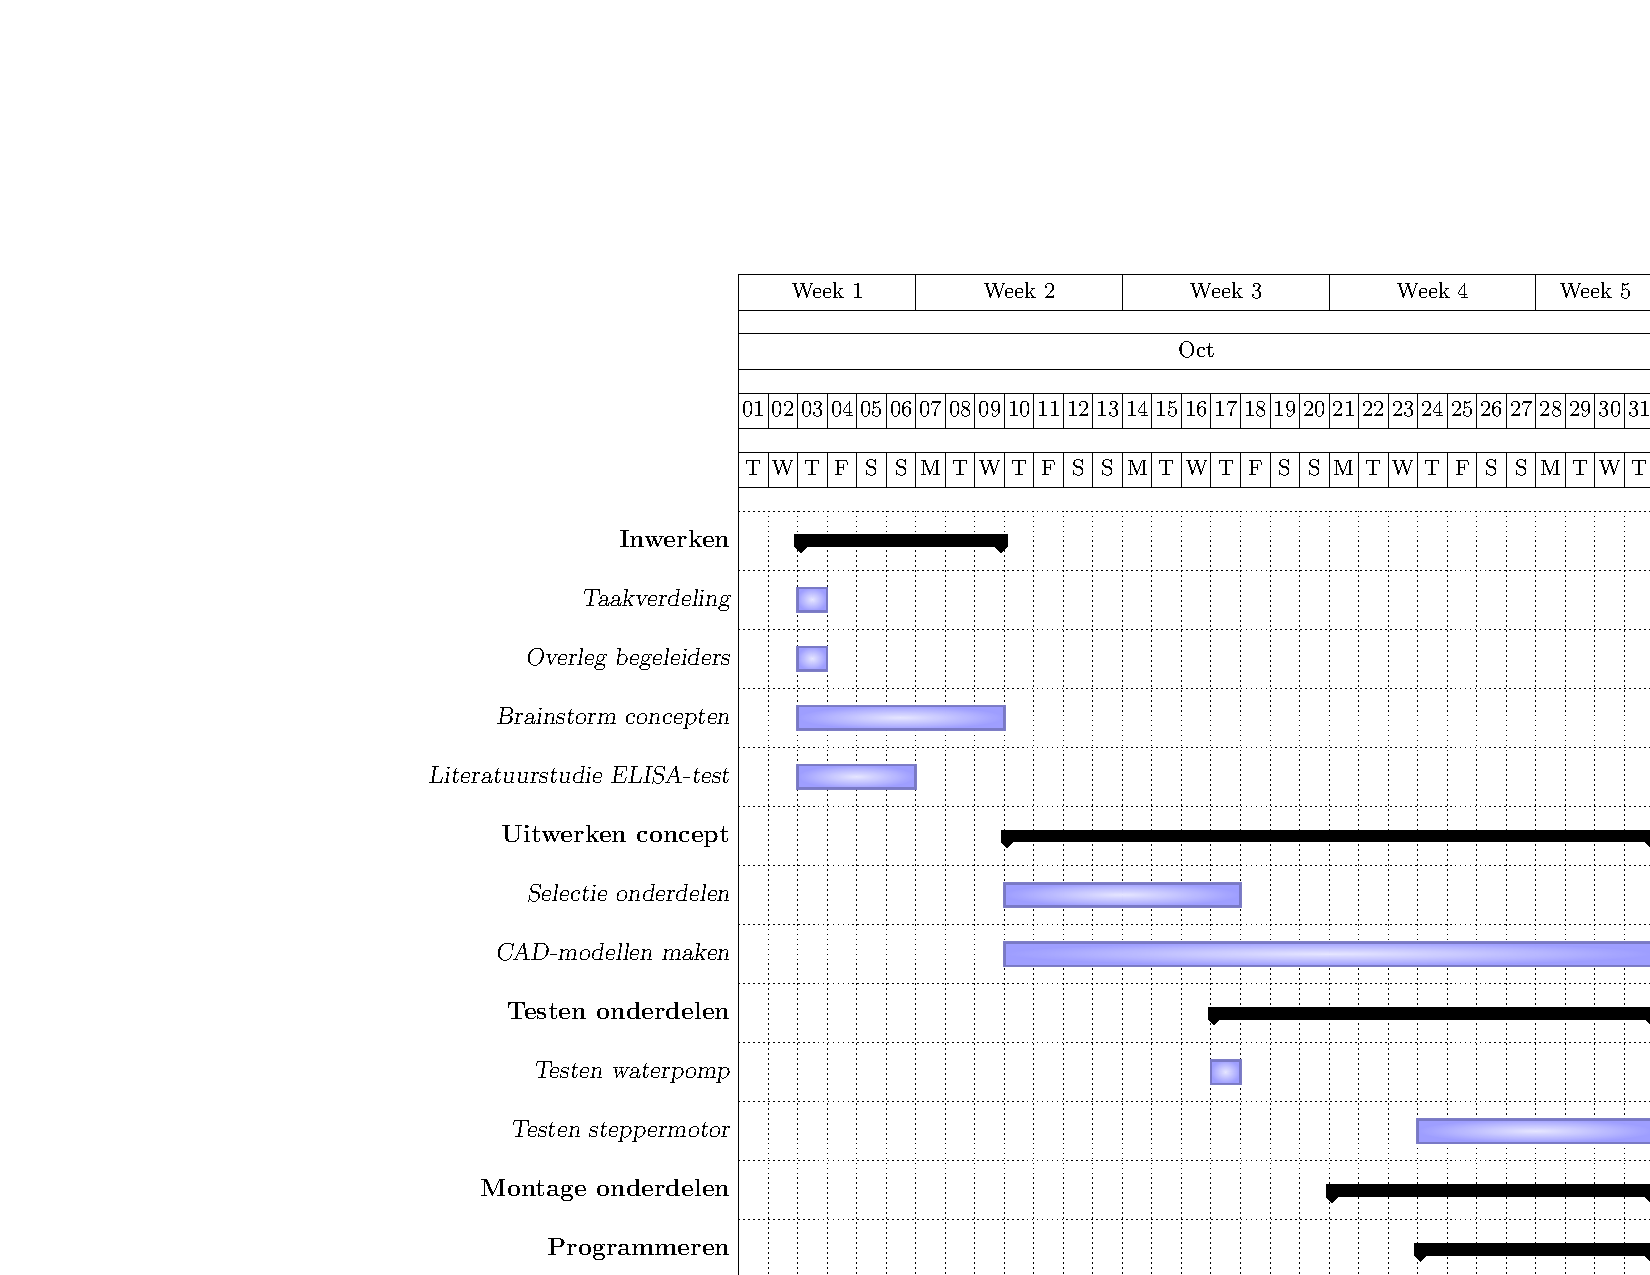
\includepdf[pages=1]{kizzigeGanttchart.pdf}
\includepdf[pages=2]{kizzigeGanttchart.pdf}
\includepdf[pages=3]{kizzigeGanttchart.pdf}


\subsection*{Vergaderverslagen}
Op de volgende pagina's vindt u de vergaderverslagen van de teambijeenkomsten.
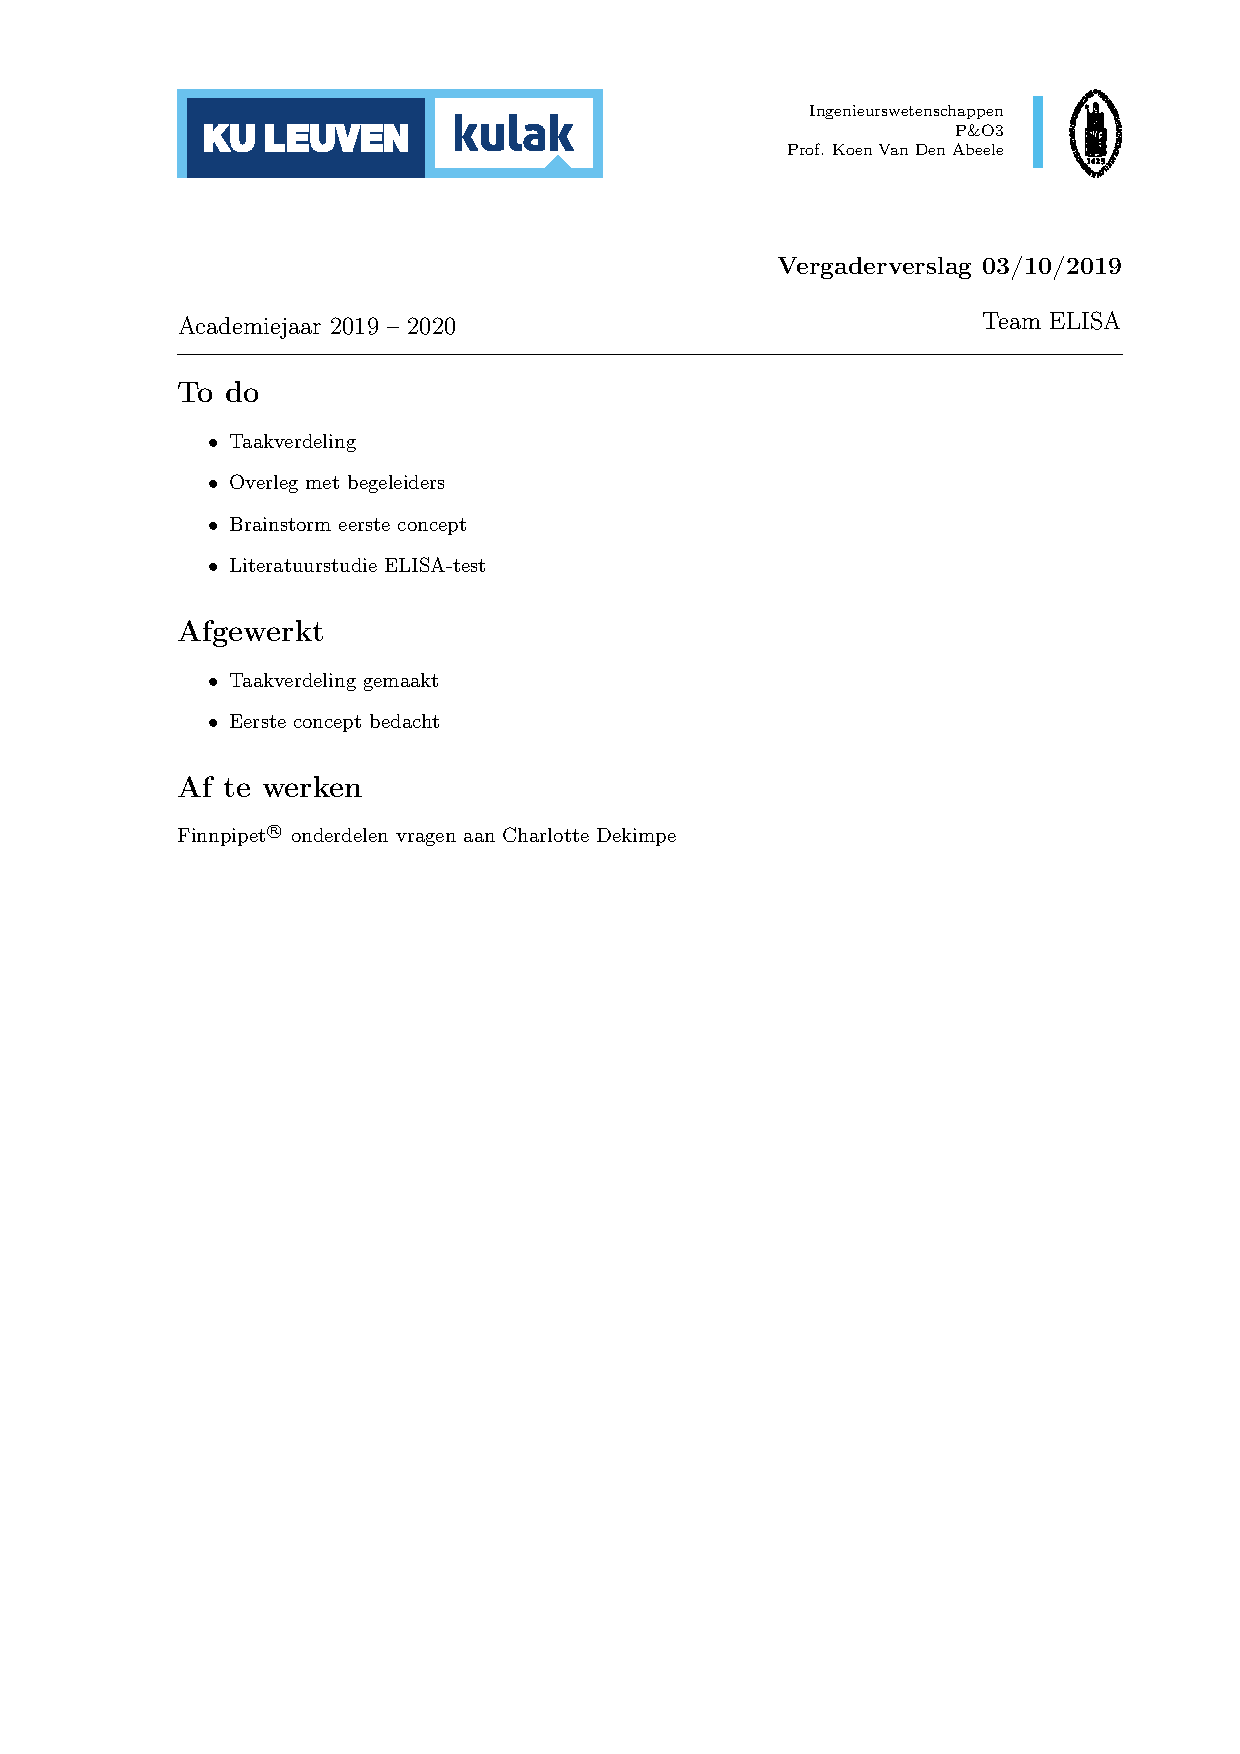
\includepdf{vergaderverslag3oktober.pdf}
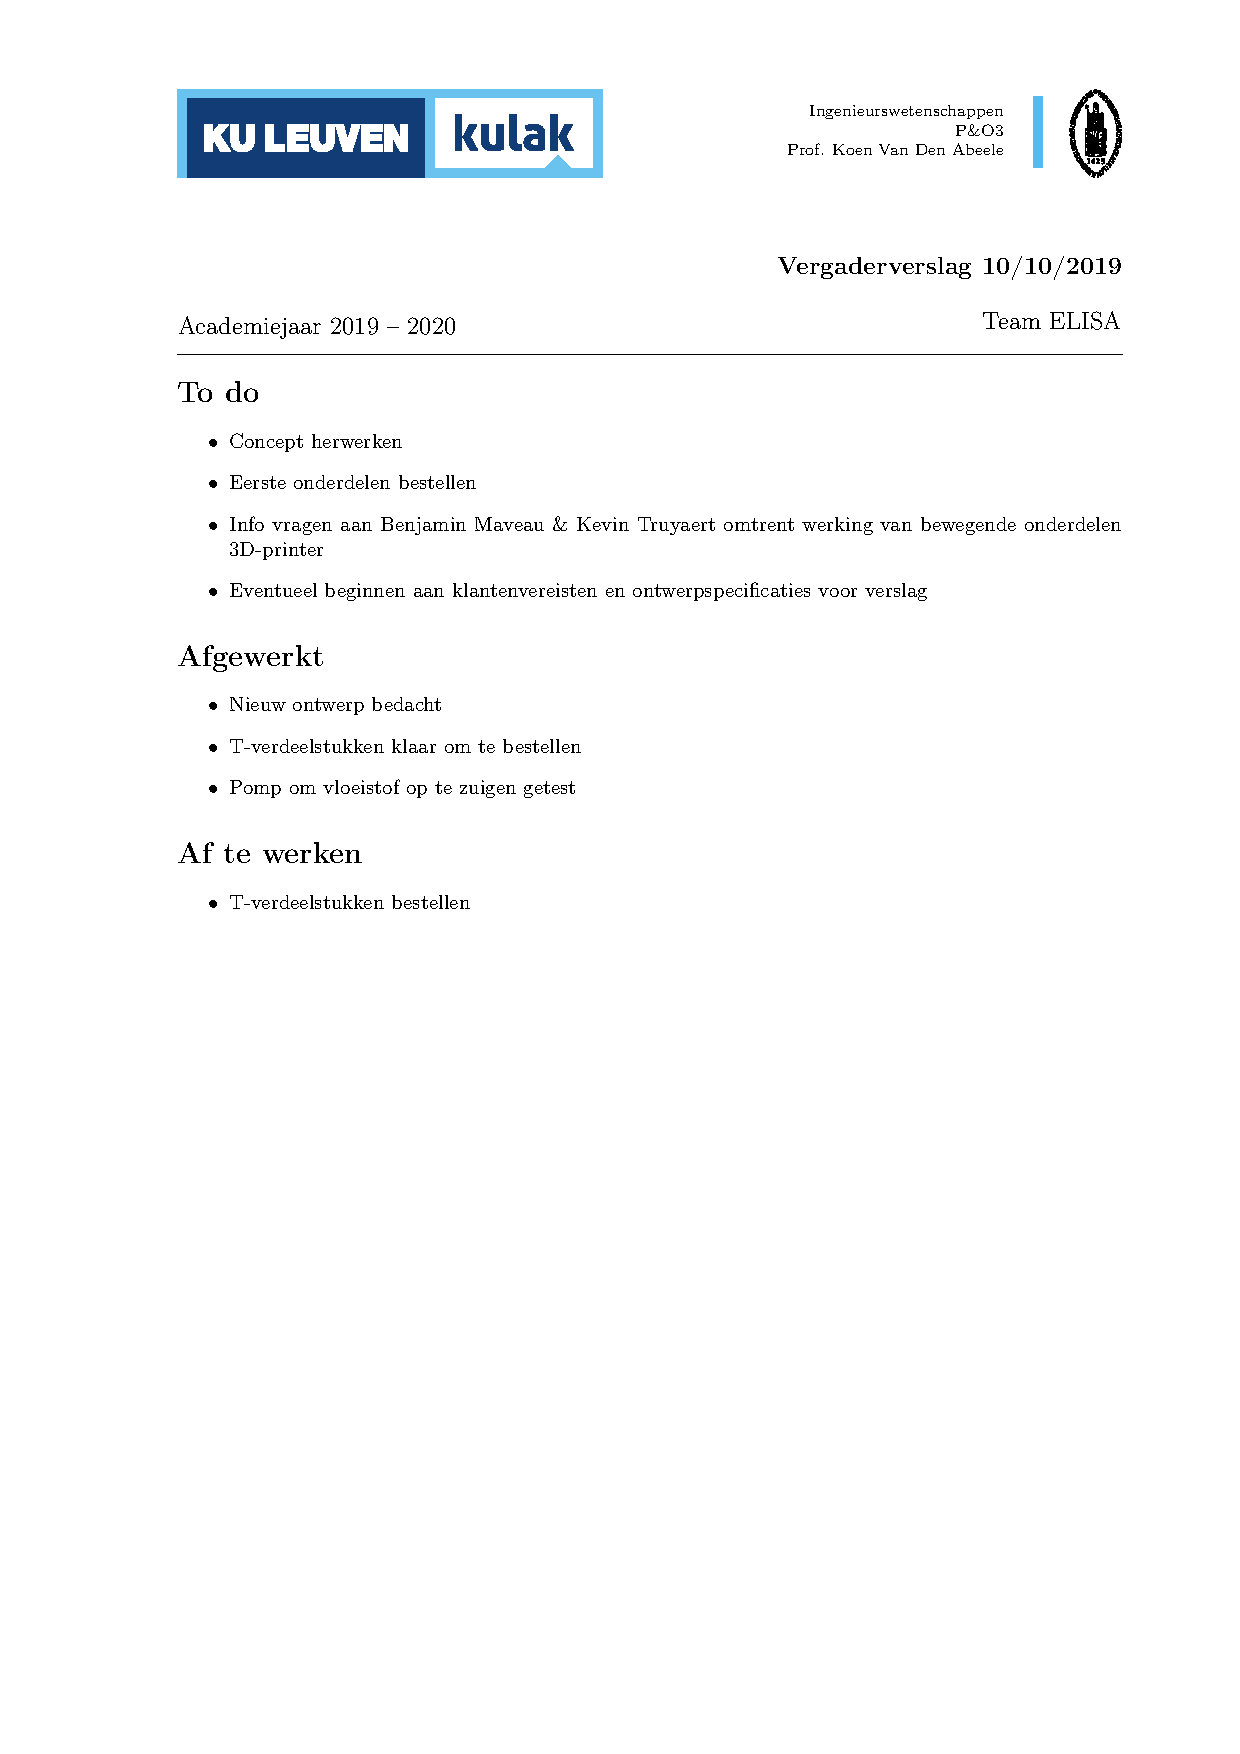
\includepdf{vergaderverslag10oktober.pdf}
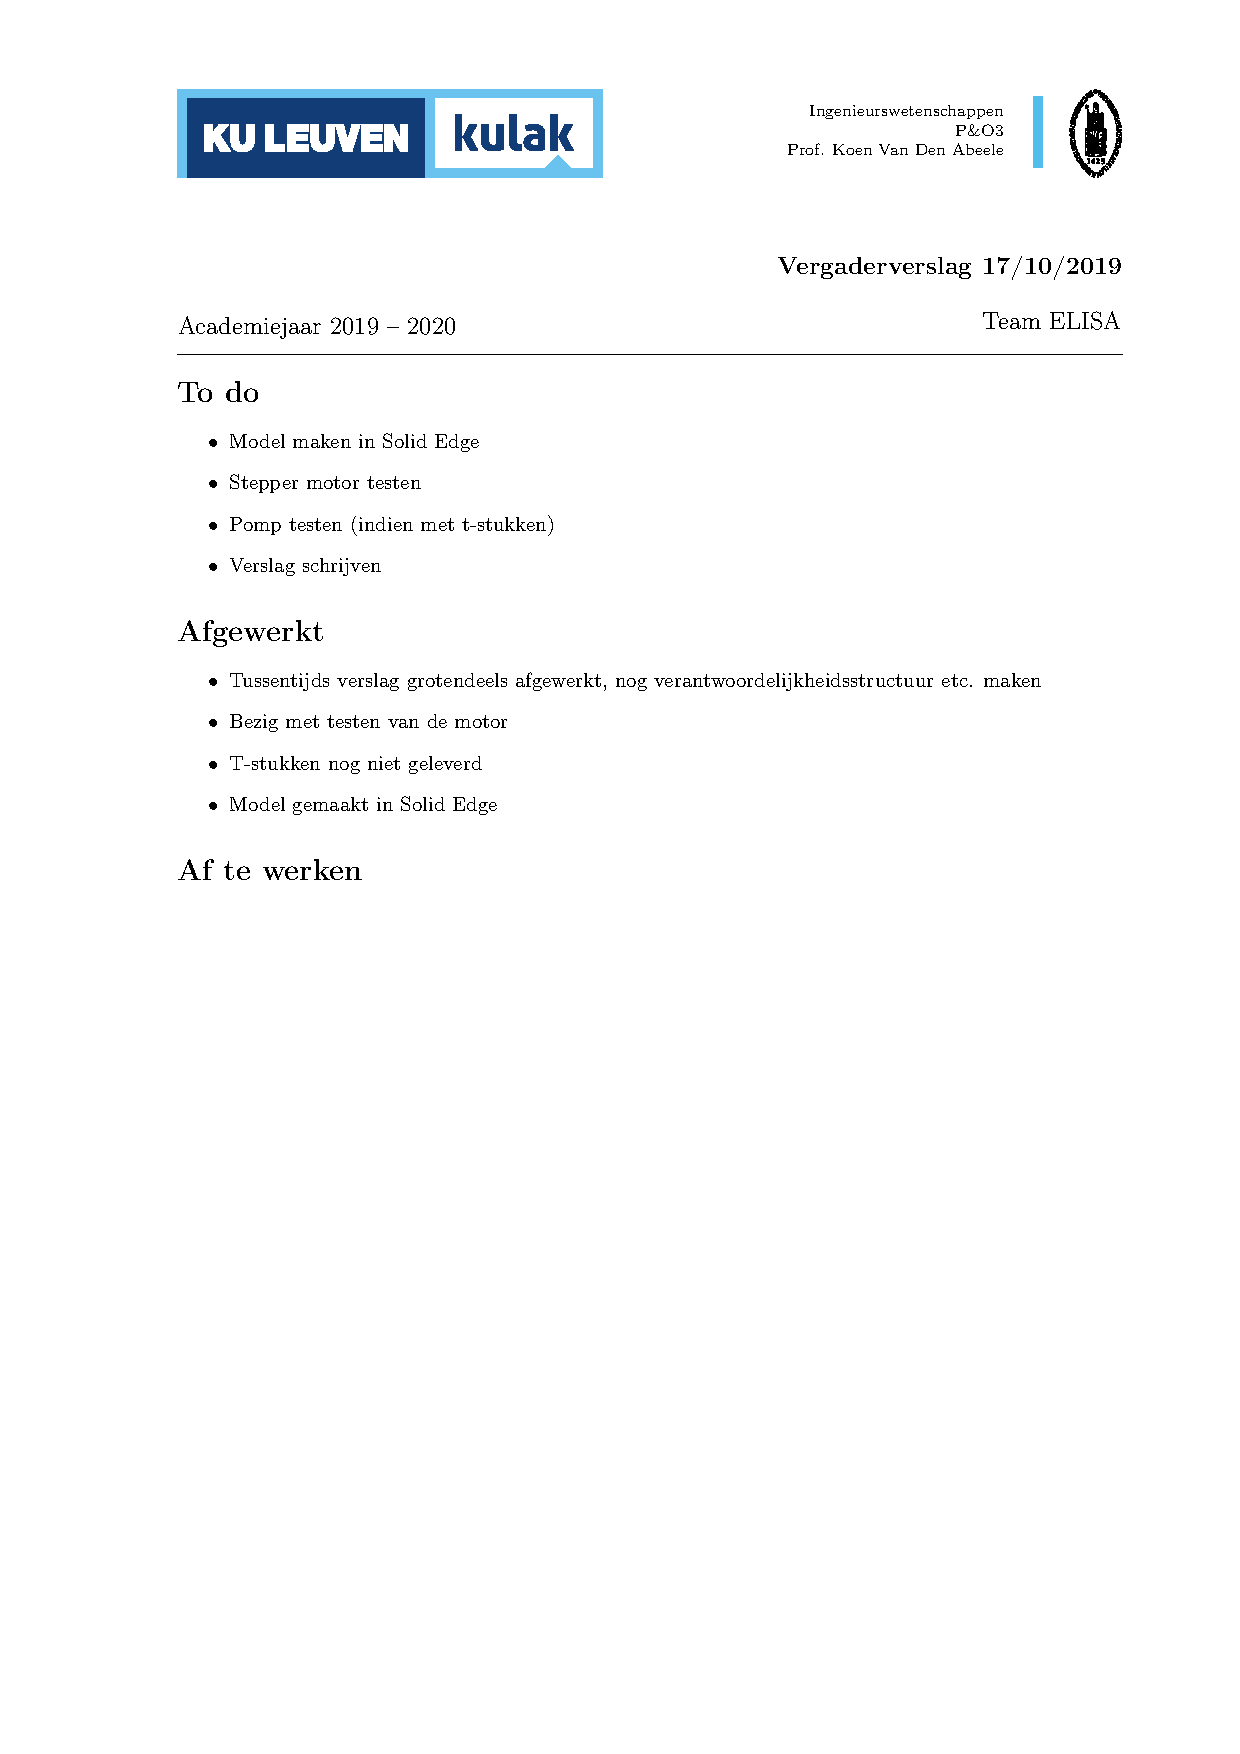
\includepdf{vergaderverslag17oktober.pdf}
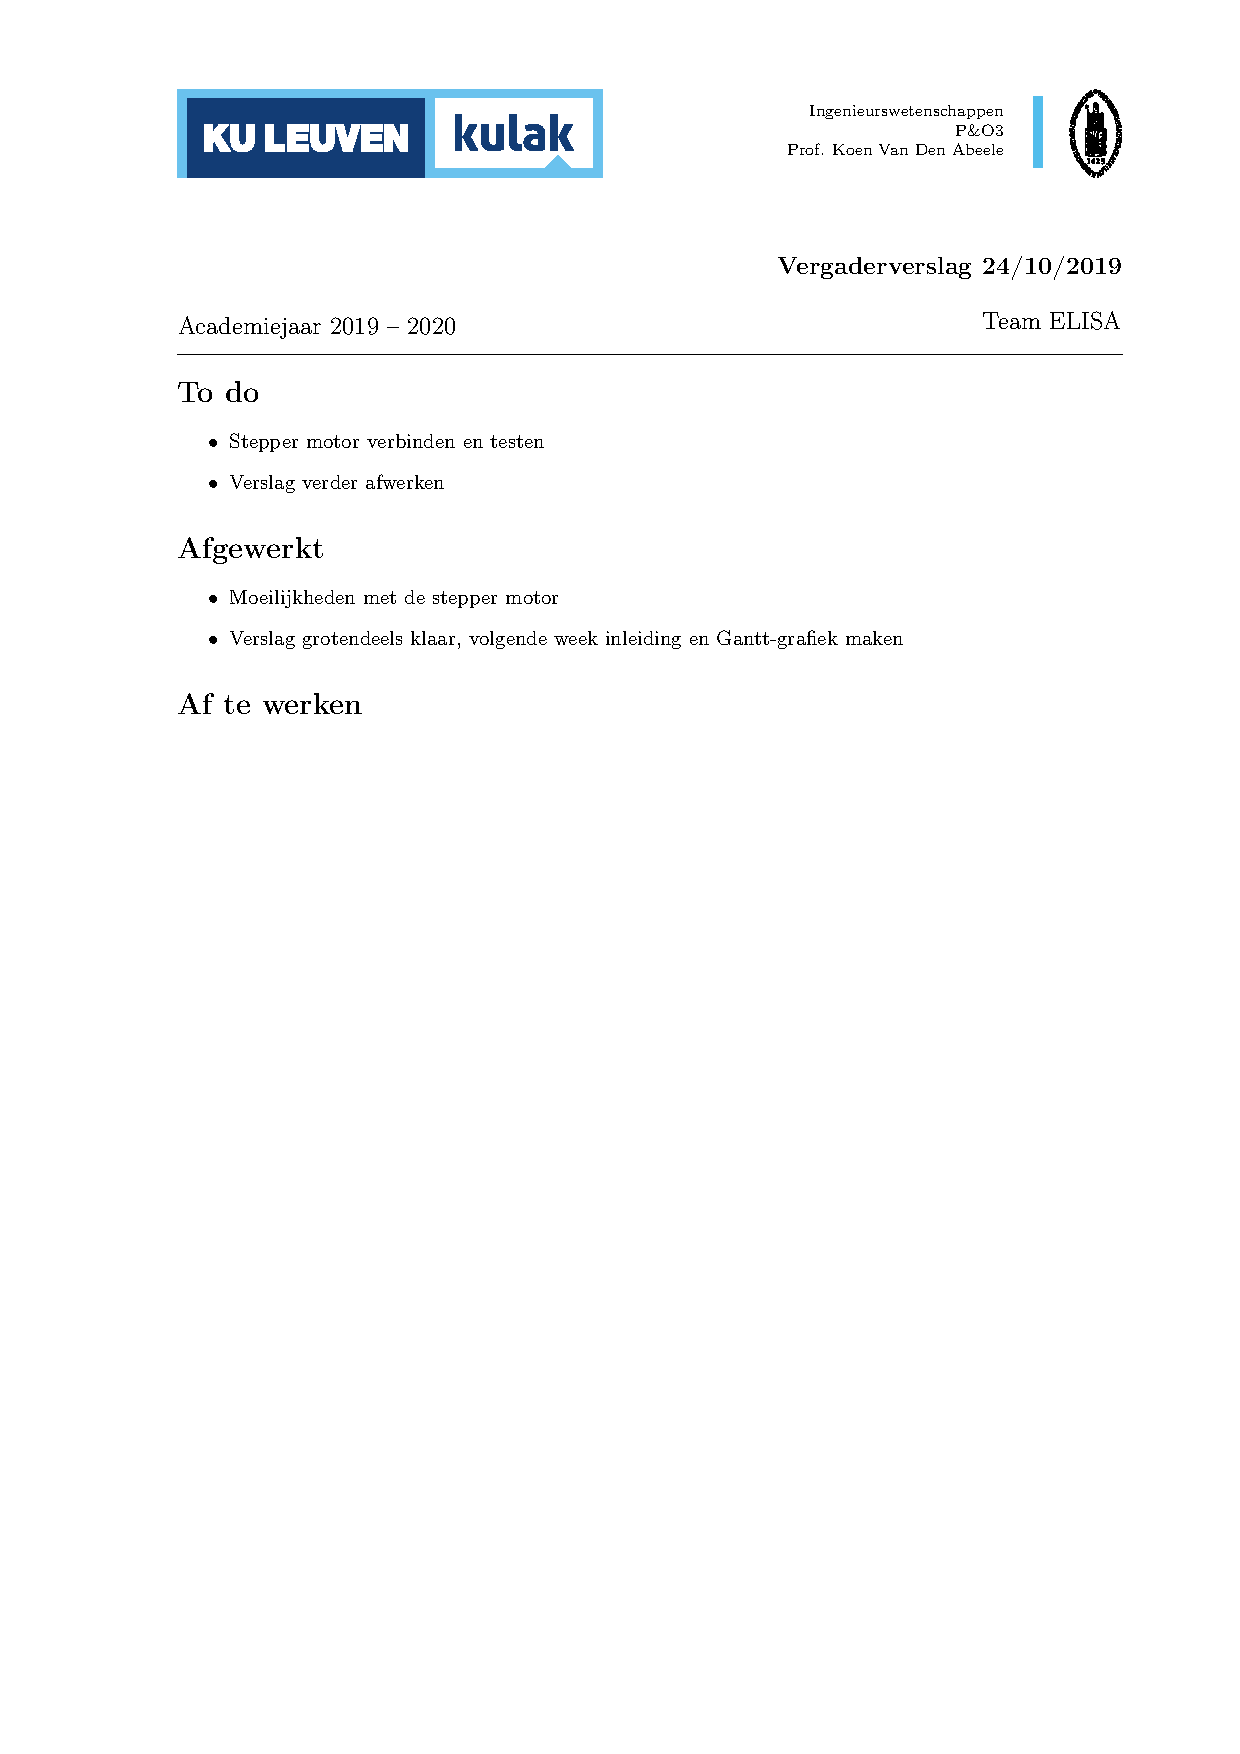
\includepdf{vergaderverslag24oktober.pdf}
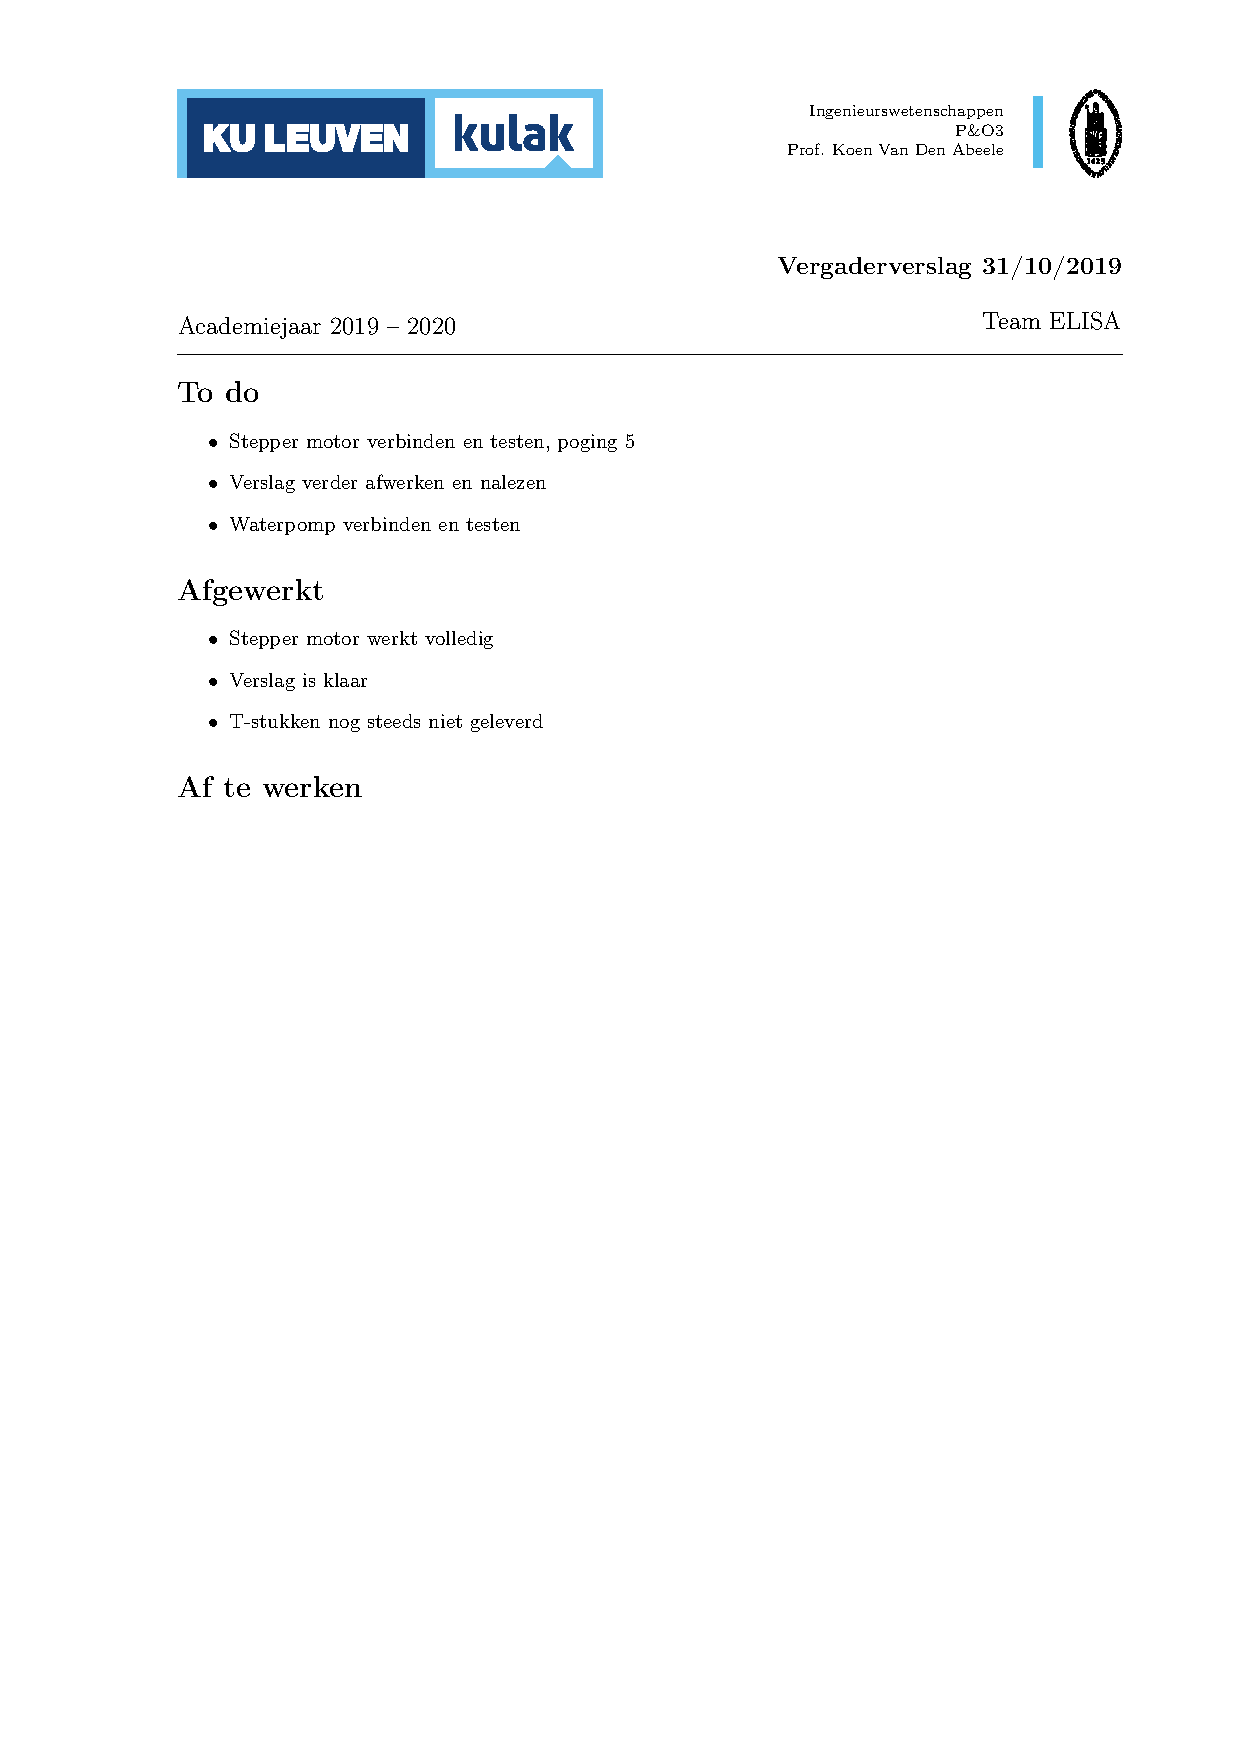
\includepdf{vergaderverslag31oktober.pdf}

 


%\clearpage
%\nocite{website:wikipedia,website:LabX}
%\bibliographystyle{plainurl}
%\bibliography{bibliografie.bib}
%\bibliographystyle{plain}


\end{document}
